% =====================================================================
%  TELFOR 2026 -- Telecommunications Forum, Belgrade, Serbia
%  Paper: Completus: Consumer-GPU QLoRA Fine-Tuning of a 1.5B Code
%         Model for Local Autocompletion
%  Authors: Nejra Smajlovic (University of Zenica, Polytechnic Faculty)
%           Adi Kadusic    (University of Zenica, Polytechnic Faculty)
%           Alen Begovic   (University of Sarajevo, Faculty of Electrical Eng.)
%
%  FORMAT COMPLIANCE (TELFOR instructions for authors):
%    * double-column A4, standard IEEE conference template (IEEEtran, 10 pt)
%    * maximum 4 A4 pages for regular and student papers
%    * submitted as PDF through the TELFOR online submission system
%
%  Figure:  python3 Telfor2026/make_figures_completus.py
%  Build:   pdflatex telfor2026_completus.tex   (run twice)
% =====================================================================
\documentclass[10pt,conference,a4paper]{IEEEtran}
\IEEEoverridecommandlockouts

\usepackage[T1]{fontenc}
\usepackage[utf8]{inputenc}
\usepackage{cite}
\usepackage{graphicx}
\usepackage{amsmath}
\usepackage{booktabs}
\usepackage{balance}
\usepackage{url}
\usepackage[hidelinks]{hyperref}
\usepackage{upgreek}   % uspravna grcka slova: IEEE ne kurzivira grcke simbole

% --- Table typography -------------------------------------------------
\newcommand{\best}[1]{\textbf{#1}}

% --- Copyright notice at the bottom of the first page ------------------
% TELFOR's Instructions for Authors do not ask for an IEEE copyright line on
% the submitted paper, and the official IEEE conference template does not
% contain one, so the paper is submitted without it rather than with a
% placeholder ISBN. If TELFOR later publishes a copyright string for the
% camera-ready version, uncomment the three lines below and paste it in.
%\IEEEpubid{\parbox{\columnwidth}{\footnotesize
%  978-1-XXXX-XXXX-X/26/\$31.00~\copyright2026 IEEE\hfill}
%  \hspace{\columnsep}\makebox[\columnwidth]{}}

\begin{document}

\title{Completus: Consumer-GPU QLoRA Fine-Tuning\\
of a 1.5B Code Model for Local Autocompletion}

\author{\IEEEauthorblockN{Nejra Smajlovi\'c}
\IEEEauthorblockA{\textit{University of Zenica}\\
\textit{Polytechnic Faculty}\\
Zenica, Bosnia and Herzegovina\\
nejra.smajlovic.22@size.ba}
\and
\IEEEauthorblockN{Adi Kadu\v{s}i\'c}
\IEEEauthorblockA{\textit{University of Zenica}\\
\textit{Polytechnic Faculty}\\
Zenica, Bosnia and Herzegovina\\
adi.kadusic.22@size.ba}
\and
\IEEEauthorblockN{Alen Begovi\'c}
\IEEEauthorblockA{\textit{University of Sarajevo}\\
\textit{Faculty of Electrical Engineering}\\
Sarajevo, Bosnia and Herzegovina\\
alen.begovic@etf.unsa.ba}%
\thanks{N. Smajlovi\'c and A. Kadu\v{s}i\'c are with the Polytechnic Faculty,
University of Zenica, and A. Begovi\'c with the Faculty of Electrical
Engineering, University of Sarajevo, Bosnia and Herzegovina. Training code,
Modelfiles and evaluation scripts:
\url{https://github.com/kadusic1/completus}.}}

\maketitle
\bstctlcite{bstctl:completus}

\begin{abstract}
This paper presents Completus, a reproducible pipeline that specialises a
1.5-billion-parameter open code model for local, network-isolated
autocompletion on a single consumer graphics card. Qwen2.5-Coder-1.5B is
fine-tuned with a fixed-rank QLoRA adapter on curated Python and Go subsets
of CodeSearchNet, after a preparation stage combining near-deduplication,
code-smell filtering, docstring quality checks and a fill-in-the-middle
transformation. The trained adapter is merged into the base weights,
exported to a four-bit K-quantised GGUF build and served through Ollama,
which makes the model reachable from a standard editor extension without any
network call. Evaluated on HumanEval under a deployment-faithful zero-shot
protocol in which the prompt is the bare function signature, the fine-tuned
Python model solves 42.68 percent of the problems on the first attempt,
against 10.98 percent for the untuned baseline under the same protocol. The
gain is therefore a recovery, in the prompt format the local deployment
actually uses, of capability the base model already reports under its own
more favourable protocol, and not a net capability increase. The complete
workflow runs on an eight-gigabyte laptop graphics card in under two hours
per language.
\end{abstract}

\begin{IEEEkeywords}
code completion, QLoRA, parameter-efficient fine-tuning, Qwen2.5-Coder,
CodeSearchNet, GGUF quantisation, local inference.
\end{IEEEkeywords}

% =====================================================================
\section{Introduction}
% =====================================================================
\IEEEPARstart{L}{arge} language models (LLMs) specialised for code deliver
accurate autocompletion and multi-file contextual awareness, but the
commercial systems that lead on those metrics are reached through
cloud-hosted endpoints. That delivery model carries three costs which are
prohibitive in regulated industries, air-gapped environments and
budget-constrained teams: a persistent network connection, exposure of
proprietary source code to third-party infrastructure, and a per-token
operational charge that never ends. A model small enough to run on the
developer's own workstation, on a single consumer graphics processing unit
(GPU), removes all three at once.

Local deployment substitutes a different constraint. The model must be
compact enough to answer within the latency budget of an editor plugin on
commodity hardware, yet capable enough that its completions are worth
accepting. Two developments make that trade-off tractable. Parameter-efficient
fine-tuning (PEFT), and in particular Low-Rank Adaptation
(LoRA)~\cite{hu2022lora}, specialises a pretrained model at a small fraction
of the cost of full fine-tuning; quantised weight formats such as GGUF,
served by optimised runtimes, execute those weights within a few gigabytes
of video memory.

This paper reports an end-to-end realisation of that recipe, named Completus,
and evaluates it in the conditions under which it is actually served. Two
gaps motivate the work. First, published studies report either raw model
capability or adaptation technique in isolation; few carry a single model
from raw corpus through data curation, adaptation and quantisation to a live,
editor-integrated endpoint, and report every stage. Second, code models are
usually scored under few-shot, chat-formatted protocols that do not resemble
the bare-signature prompts an editor plugin emits, so a published score does
not predict what a developer will experience. The contributions are the
complete pipeline of Fig.~\ref{fig:pipeline}, reported with the parameters
needed to reproduce it; a quantification of the effect of a single QLoRA
epoch measured in the deployment prompt format; and an explicit separation of
capability recovery from capability gain, which the evaluation protocol
determines and which published scores routinely conflate.

\begin{figure*}[!t]
\centering
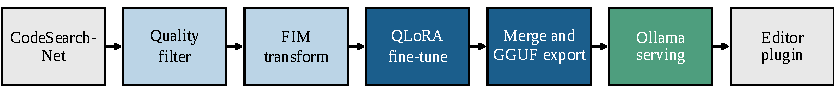
\includegraphics[width=\textwidth]{figures/fig_pipeline.pdf}
\caption{The Completus pipeline. Raw CodeSearchNet functions pass through
quality filtering and a fill-in-the-middle transform, specialise
Qwen2.5-Coder-1.5B through QLoRA, and are merged and exported to a four-bit
K-quantised GGUF build that Ollama serves to an editor plugin over the
local loopback interface.}
\label{fig:pipeline}
\end{figure*}

% =====================================================================
\section{Related Work}
% =====================================================================
Building on the decoder-only Transformer~\cite{vaswani2017}, a succession of
open code models has narrowed the gap to proprietary systems.
StarCoder~\cite{li2023starcoder} trains on the permissively licensed Stack
corpus with multi-query attention and a fill-in-the-middle (FIM) objective;
Code Llama~\cite{roziere2023} extends Llama~2 with infilling and long-context
support; DeepSeek-Coder~\cite{guo2024} trains on a project-level corpus with
an infilling objective; and Qwen2.5-Coder~\cite{hui2024} reports the leading
scores among open models at the 1.5-billion-parameter scale adopted here.
Completus differs in goal rather than in technique: it does not pretrain a
new model but specialises an existing small one for a narrow,
latency-sensitive task.

On the adaptation side, LoRA~\cite{hu2022lora} freezes the pretrained
weights and injects trainable rank-decomposition matrices, cutting trainable
parameters by orders of magnitude. Quantized LoRA (QLoRA)~\cite{dettmers2023}
quantises the frozen base to four-bit NormalFloat (NF4), which brings
fine-tuning within the memory budget of a single consumer card.
AdaLoRA~\cite{zhang2023adalora} refines the allocation of rank by importance.
Weyssow \emph{et al.}~\cite{weyssow2025} evaluate PEFT specifically for code
generation and confirm that LoRA recovers most of the quality of full
fine-tuning at a fraction of its cost, and the survey of Han \emph{et
al.}~\cite{han2024} situates LoRA within the wider PEFT family.

A third line concerns the training data. Xue \emph{et al.}~\cite{xue2025}
show that removing code smells from the training set improves model quality;
Lee \emph{et al.}~\cite{lee2022} that near-deduplication reduces memorisation
and test-set leakage; Bavarian \emph{et al.}~\cite{bavarian2022} that models
acquire infilling ability at no cost to left-to-right generation; and
WizardCoder~\cite{luo2024} that instruction-style tuning lifts code quality
further. The quantisation build follows the unified evaluation of llama.cpp
formats by Kurt~\cite{kurt2026}. What these works share is that each is
developed and reported in a research or cloud-serving setting, under a
protocol chosen by its own authors. None delivers a recipe that carries a
small open model all the way to an editor-integrated endpoint on commodity
hardware, and reports its quality in the prompt format that endpoint receives.


% =====================================================================
\section{The Completus Pipeline}
% =====================================================================
The pipeline has five stages, shown in Fig.~\ref{fig:pipeline}: data
preparation, QLoRA fine-tuning, adapter merging, GGUF export and local
registration for serving. Each stage is scripted and parameterised, so that
the whole path from public corpus to running endpoint can be re-executed on
one machine.


\subsection{Data Preparation}
The corpus is CodeSearchNet~\cite{husain2019}, whose full splits contain
412\,178 Python and 317\,832 Go functions. To keep preparation tractable on
one workstation the input is capped at the first 50\,000 functions per
language, which are then passed through five filters. Near-duplicates are removed by
locality-sensitive hashing over MinHash sketches (128 permutations,
five-token shingles, Jaccard threshold 0.8). A code-smell filter drops lines
over 120 characters, functions under 30 tokens, and bodies that do nothing. A docstring filter requires at least 15
tokens and two words and rejects any docstring carrying a TODO, FIXME or XXX
marker. A fill-in-the-middle transform is then applied to 80~\% of the
surviving samples, and the remainder are truncated to 2048 tokens.

Each filter targets a documented failure mode. Near-deduplication is applied
because duplicated text increases memorisation and leaks test material into
training~\cite{lee2022};
the code-smell filter because models trained on smell-cleaned corpora produce
better code~\cite{xue2025}; and the FIM transform because it buys infilling
ability, which is what an editor plugin needs, at no measured cost to
left-to-right generation~\cite{bavarian2022}.

Table~\ref{tab:data} reports what survives. Retention differs sharply
between the two languages, 63.9~\% for Python against 42.6~\%~for Go, and
the gap is dominated by the docstring filter, since idiomatic Go comments are
frequently shorter than the 15-token floor. The consequence is that the two
adapters are not trained on comparable amounts of data, which must be kept in
view when the two models are compared.

\begin{table}[b]
\caption{Training data surviving the preparation pipeline}
\label{tab:data}
\centering
\footnotesize
\begin{tabular}{@{}lrrr@{}}
\toprule
\textbf{Language} & \textbf{Input cap} & \textbf{After pipeline} & \textbf{Retained}\\
\midrule
Python & 50\,000  & 31\,966 & 63.9~\%\\
Go     & 50\,000  & 21\,284 & 42.6~\%\\
\midrule
Total  & 100\,000 & 53\,250 & 53.3~\%\\
\bottomrule
\end{tabular}
\end{table}

\subsection{QLoRA Fine-Tuning}
Qwen2.5-Coder-1.5B~\cite{hui2024} is loaded in four-bit NF4 quantisation and
adapted with QLoRA~\cite{dettmers2023} through the Unsloth runtime. Adapters
are attached to all seven linear projection matrices, at a fixed rank rather
than an adaptively allocated one, so that the memory ceiling is known in
advance on an eight-gigabyte card. Table~\ref{tab:config} lists the full
configuration.

\begin{table}[b]
\caption{QLoRA fine-tuning configuration}
\label{tab:config}
\centering
\footnotesize
\begin{tabular}{@{}ll@{}}
\toprule
\textbf{Parameter} & \textbf{Value}\\
\midrule
Base model                & Qwen2.5-Coder-1.5B\\
Quantisation              & four-bit NF4\\
LoRA rank / scaling       & 16 / 32\\
Target modules            & q, k, v, o, gate, up, down\\
Batch size / accumulation & 2 / 8 (effective 16)\\
Learning rate / schedule  & 0.0002 / cosine\\
Optimiser                 & AdamW, eight-bit\\
Epochs / max.\ seq.\ length & 1 / 2048\\
Random seed               & 3407\\
Hardware                  & NVIDIA RTX 4060 Laptop (8\,GB)\\
\bottomrule
\end{tabular}
\end{table}

The eight-gigabyte budget is what dictates that configuration. Fine-tuning
every parameter of a model this size in mixed precision needs on the order of
16 bytes per parameter once half-precision weights, their gradients, a
single-precision master copy and the two AdamW moments are all resident,
which is roughly 24\,GB, or three times what the card offers. QLoRA removes
almost all of it: the frozen base held in four-bit NF4 occupies under a
gigabyte, and since only the injected low-rank matrices are trained,
gradients and optimiser state exist for a small fraction of the parameters,
halved again by the eight-bit optimiser. What remains of the budget is spent
on activations, whose peak is set by the 2048-token sequence length and the
micro-batch. That is why the batch is split into two samples with eightfold
gradient accumulation rather than sixteen at once: the split leaves the
effective batch size unchanged while keeping the activation peak inside the
card, and it is the setting that decides whether the run fits at all.

Each language is trained for a single epoch: 1998 optimiser steps for Python
and 1331 for Go at an effective batch size of 16. The Go run completed in
3713~s (62~min) and the Python run in approximately 2.2~h, so a full
language fits inside a working session on a laptop. Training loss falls from
1.674 at the start of the Python run, and the Go run ends at a mean training
loss of 1.111.

\subsection{Merging, Export and Local Serving}
After training, the LoRA weights are merged into the base checkpoint and
exported as a quantised GGUF binary in the \texttt{q4\_k\_m}
scheme, which the unified evaluation of llama.cpp
formats~\cite{kurt2026} identifies as a favourable size-quality compromise,
although that evaluation covers an eight-billion-parameter model, so its
conclusions are carried to a smaller one unverified. The K-quant schemes are not uniform four-bit formats: \texttt{q4\_k\_m}
keeps part of the attention value and feed-forward projections at six bits
and rounds the remainder to four, spending the extra bits where the accuracy
cost of rounding is highest. That non-uniformity, rather than the nominal bit
width, is what makes it the usual choice at this quantisation level.

Each binary is
registered with Ollama through a Modelfile that fixes the FIM prompt
template, a decoding temperature of 0, a context window of 2048 tokens and a
generation limit of 256 tokens. The result is an endpoint on the local
loopback interface, consumed directly by the Continue.dev editor extension;
no request leaves the machine.

\subsection{Hardware Constraints on Local Serving}
Quantisation matters for serving, not only for fitting, and the reason lies
in the device rather than in the model. Autoregressive decoding at a batch
size of one reduces every weight matrix to a matrix-vector product in which
each weight is read once and used once. No reuse remains for the tensor units
to exploit, so arithmetic intensity falls to about one operation per byte and
the decode rate is set by memory bandwidth, not by arithmetic throughput.

The ceiling is therefore calculable in advance. The card used here couples
8\,GB of GDDR6 to a 128-bit bus at 16\,Gbit/s per pin, giving 256\,GB/s. The
\texttt{q4\_k\_m} build of a 1.54-billion-parameter model occupies about
1\,GB, so no more than roughly 250 tokens per second can be emitted even with
the memory system saturated; the merged half-precision checkpoint occupies
3.1\,GB and is bounded near 80. The factor of three between them is a
bandwidth effect, not a reduction in the number of operations performed.

Two terms qualify that bound in opposite directions. The key-value cache is
read alongside the weights, some 28\,kB per token for this architecture, so a
full 2048-token window adds about 60\,MB per step, under a tenth of the
weight traffic. Against that, K-quantised blocks must be unpacked before they
can be multiplied, spending arithmetic the half-precision path does not, so
the realised speed-up is smaller than the traffic ratio suggests. Prefill
differs again: the prompt is consumed in one pass, which restores reuse and
makes that phase compute-bound, so time to a first suggestion and the
interval between tokens are limited by different parts of the device.

All of the above are bounds derived from published device and model
parameters, not measurements; Section~\ref{sec:limits} records that the
realised figures were not collected.

% =====================================================================
\section{Evaluation}
% =====================================================================
\subsection{Protocol}
Evaluation uses HumanEval, whose 164 Python problems each pair a function
signature with hidden unit tests. Generation is greedy, one deterministic
sample per problem and at most 512 new tokens, and the reported metric is
pass@1: the fraction of problems whose generated body passes every test.

Only pass@1 is reported. Counting a problem solved if any of several
sampled completions passes measures a property no editor plugin exposes: the
developer sees one suggestion and accepts it or does not. Greedy pass@1
therefore measures what the deployment delivers, at the cost of a wider
confidence interval.

The prompt matters more than the decoding here. Rather than the few-shot,
chat-formatted prompt used in the base model's own report, the prompt is the
bare function signature, which is what an editor plugin sends. Both
checkpoints are evaluated under identical conditions, so the comparison
between them is internally valid even though neither number is comparable to
a published score obtained under a different protocol. Because decoding is
deterministic, the only source of uncertainty is the finite problem set, and
95~\% Wilson confidence intervals (CIs) are reported accordingly.

\subsection{Results}
The fine-tuned Python model solves 70 of the 164 problems, a pass@1 of
42.68~\% with a 95~\% confidence interval of [35.4, 50.3]. The untuned
baseline solves 18, a pass@1 of 10.98~\% with an interval of [7.1, 16.7].
The intervals do not overlap, so the difference of 31.7 percentage points is
distinguishable from sampling noise under this protocol.

\subsection{Reading the Result Against Published Scores}
The interpretation of that difference depends entirely on what the baseline
number measures. Under its own few-shot protocol, the same base model is
reported at 43.9~\%~\cite{hui2024} --- almost exactly what the fine-tuned
model reaches here. The 10.98~\% baseline therefore does not describe a weak
model; it describes a capable model penalised by a prompt format it was not
prepared for. One QLoRA epoch teaches it to emit a function body directly
from a signature, which recovers that latent capability in the format the
deployment uses. Table~\ref{tab:humaneval} places both numbers next to
published scores for comparable models; those scores were obtained under
protocols set by their own authors and are context, not a controlled
comparison.

\begin{table}[b]
\caption{HumanEval pass@1. The upper block is measured here under a single
protocol; the lower block reproduces published scores obtained under
protocols that differ from it and from each other}
\label{tab:humaneval}
\centering
\footnotesize
\begin{tabular}{@{}llrl@{}}
\toprule
\textbf{Model} & \textbf{Params} & \textbf{pass@1} & \textbf{95~\% CI}\\
\midrule
\multicolumn{4}{@{}l}{\emph{Measured here, bare-signature zero-shot protocol}}\\
Qwen2.5-Coder-1.5B (baseline) & 1.5B & 10.98~\% & [7.1, 16.7]\\
Completus Python (fine-tuned) & 1.5B & \best{42.68~\%} & [35.4, 50.3]\\
\midrule
\multicolumn{4}{@{}l}{\emph{Published, each under its own protocol}}\\
CodeLlama-Base~\cite{guo2024}       & 7B    & 31.7~\% & ---\\
StarCoderBase~\cite{guo2024}        & 15.5B & 31.7~\% & ---\\
DeepSeek-Coder-Base~\cite{guo2024}  & 1.3B  & 34.8~\% & ---\\
Qwen2.5-Coder base~\cite{hui2024}   & 1.5B  & 43.9~\% & ---\\
\bottomrule
\end{tabular}
\end{table}

% =====================================================================
\section{Discussion and Threats to Validity}
\label{sec:limits}
% =====================================================================
The practical reading is that a compact open model, adapted for two hours
on a laptop card, serves autocompletion at a quality close to what its
publishers report, with no network dependency and no per-token cost. What the
fine-tuning buys is not intelligence but format alignment, and that
distinction is the paper's main methodological point: a benchmark score is a
property of a model and a prompt protocol jointly, so a score obtained under a
favourable protocol does not transfer to a deployment that prompts
differently. That argues for evaluating under the protocol a system will
actually receive.

For a team weighing a hosted endpoint against a local one, the cost of
going local is one laptop-class card and two hours of training per language.
Table~\ref{tab:humaneval} also shows that model size is not the whole story
at this scale: the adapted 1.5-billion-parameter model reaches a score
comparable to published figures for models four to ten times larger, though
under protocols that differ and therefore only as an indication.

Five limitations bound these results. First, only the Python model is
evaluated quantitatively; the Go model is assessed qualitatively, so the
retention gap reported in Section~III-A is not tied to a measured quality
difference. Second, HumanEval scores self-contained function synthesis, not
the cursor-aware infilling that the FIM objective trains and that the editor
plugin actually issues, so the reported figure does not measure the deployed
task directly. Third, the pipeline input is capped at 50\,000 functions per
language and the filter thresholds are fixed, so the retention rates are a
single operating point rather than a tuned optimum. Fourth, one training run
per language was executed under a fixed seed, so run-to-run variance is not
quantified. Fifth, and most relevant to the stated motivation, the deployed
artefact is bounded analytically in Section~III-D but never measured: no
completion latency, throughput or inference memory footprint is reported, and
the effect of four-bit quantisation on answer quality is not separated from
that of the fine-tuning.

% =====================================================================
\section{Conclusion}
% =====================================================================
Completus carries a 1.5-billion-parameter open code model from a public
corpus to an editor-integrated endpoint that runs entirely on an
eight-gigabyte consumer card, and reports every stage of that path. A single
QLoRA epoch raises HumanEval pass@1 from 10.98~\% to 42.68~\% under a
bare-signature zero-shot protocol, approaching the 43.9~\% the base model
reports under its own more favourable protocol. That result is best read as
recovery rather than gain: the fine-tuning aligns the model with the prompt
format the deployment emits, and the size of the effect is a measure of how
much a protocol mismatch can suppress an otherwise capable model. Future work will
measure the served endpoint against the bounds of Section~III-D, evaluate the
Go model on HumanEval-X, and adopt an infilling-aware benchmark matching the
deployed usage.

\section*{Acknowledgment}
This paper is based, in part, on research conducted during the first and
second authors' ongoing master's studies in Software Engineering at the
University of Zenica, focusing on data mining.

\balance

% =====================================================================
\bibliographystyle{IEEEtran}
\bibliography{refs_completus}

\end{document}
